\documentclass{beamer}
\usetheme[]{default}
\usecolortheme{beaver}
\usepackage{tikz}
\usepackage{multirow}

\beamertemplatenavigationsymbolsempty %suppress navigation bar

%\addtobeamertemplate{frametitle}{}

%TITLEPAGE
\title[Imputing squares] {Multiple Imputation of Squared Terms}
%\author[Vink, Van Buuren]
%{
%  Gerko~Vink\inst{1,2} \and
%  Stef~Van Buuren\inst{1,3} \and
%}
%
%\institute[Utrecht University and others]
%{
%  \inst{1}%
%  Utrecht University
%  \and
%  \vskip-2mm
%  \inst{2}%
%  Statistic Netherlands
%  \and
%  \vskip-2mm
%  \inst{3}%
%  Netherlands Organization for Applied Scientific Research TNO
%  \vskip6mm
%}

\author[Vink, Van Buuren]
{
  Gerko~Vink \and
  Stef~van Buuren
}


\date[ISA 2014]
{XVIII ISA World Congress of Sociology \vskip6mm}



\begin{document}


%%%%
%\begin{frame}
\titlepage
\begin{tikzpicture}[remember picture,overlay]
\node[anchor=south, yshift=2pt] at (current page.south) {
\includegraphics[height=0.6cm] {UU.png} 
\includegraphics[height=0.6cm]{TNO.png} 
\includegraphics[height=0.6cm]{CBS.png}\hspace{.25 in}};
\end{tikzpicture}
%\end{frame}


%%%%
\begin{frame}
  \frametitle{Some introduction}
  
  \begin{itemize}
  \item Multiple imputation (MI)\footnote{\tiny{Rubin, D. B. (1987). Multiple imputation for nonresponse in surveys. New York: Wiley.}}
 	  \begin{itemize}
	  \item A general and valid approach for dealing with missing data
	  \item Widely accepted and well documented for a variety of problems and situations. 
	  \item Can be very flexible
	  \end{itemize} \vspace{.25 in}
  \item MI requires {\bf correct} specification of the imputation model	  
   	  \begin{itemize}
	  \item Straightforward when the analysis model contains main effects
	  \item Less clear when nonlinear terms are included
	  \end{itemize}
  \end{itemize}
 \end{frame}
 
%%%%
\begin{frame}
  \frametitle{Adding nonlinear terms}
  \begin{itemize}
  \item Take the following model of scientific interest
\begin{equation*}\label{Y}
Y = \alpha + X \beta_1 + X^2 \beta_2 + \epsilon
\end{equation*}
\item If we want to predict Y from X and its square $X^2$ , then both X and $X^2$ should be included in the imputation model. 
\item Leaving the term $X^2$ out of the imputation model will result in a downward bias of the slopes when we perform a regression analysis on the imputed data.
  \end{itemize}
 \end{frame}
 
%%%%
\begin{frame}
  \frametitle{Imputing squares: Option\footnote{\tiny{These options have been studied by Paul von Hippel in Von Hippel, P. (2009) How to Impute Interactions, Squares, and Other Transformed
Variables. Sociological Methodology 39:265-91.}} 1}
  \begin{itemize}
  \item Transform, then impute
  \begin{itemize}
  \item Transform $X$ in the incomplete data and impute $X^2$ as just another variable.
  \item Yields unbiased regression estimates under MCAR
  \item Heavily distorts the relation between $X$ and $X^2$ after imputation. 
  \end{itemize}
  \end{itemize}
  \vspace{0.2 in}
\resizebox{\textwidth}{!}{  
\begin{tabular}{lcccccrl}
\hline
&\multicolumn{5}{c}{Missingness Mechanism} \\
\cline{2-6}
							&MCAR	&MARleft	&MARmid		&MARtail	& MARright\\
 \hline
%\textit{Polynomial combination}	&&&&&\\
%Intercept ($\alpha$)				&0		&-0.01	&-0.01	&-0.05	&-0.07\\
%Slope of $X$ ($\beta_1$)			&1		&1		&1		&0.96	&0.96\\	
%Slope of $X^2$ ($\beta_2$)		&1		&1		&1.01	&1.06	&1.09\\	
%Residual SD ($\sigma_\epsilon$) 	&1		&1		&1		&1.03	&1.05\\	
%$R^2$						&0.75	&0.75	&0.75	&0.73	&0.73\\\\
%\textit{Impute, then transform}	&&&&&\\
%Intercept ($\alpha$)				&0.39	&0.29	&0.26	&0.52	&0.56\\
%Slope of $X$ ($\beta_1$)			&0.93	&0.94	&0.87	&1.01	&1.06\\
%Slope of $X^2$ ($\beta_2$)		&0.61	&0.60	&0.67	&0.56	&0.66\\
%Residual SD ($\sigma_\epsilon$) 	&1.48	&1.44	&1.41	&1.56	&1.62\\
%$R^2$						&0.45	&0.48	&0.5		&0.39	&0.34\\\\
%\textit{Passive imputation}	&&&&&\\
%Intercept ($\alpha$)				&0.39	&0.29	&0.26	&0.52	&0.56\\
%Slope of $X$ ($\beta_1$)			&0.93	&0.94	&0.87	&1.01	&1.05\\
%Slope of $X^2$ ($\beta_2$)		&0.61	&0.60	&0.68	&0.56	&0.66\\
%Residual SD ($\sigma_\epsilon$) 	&1.48	&1.45	&1.41	&1.57	&1.62\\
%$R^2$						&0.45	&0.48	&0.50	&0.38	&0.34\\\\
\textit{Transform, then impute}	&&&&&\\
Intercept ($\alpha$)				&0		&0.19	&-0.13	&0.01	&-0.05\\
Slope of $X$ ($\beta_1$)			&1		&0.91	&0.97	&1.14	&1.32\\
Slope of $X^2$ ($\beta_2$)		&1		&0.91	&0.95	&1.14	&1.32\\
Residual SD ($\sigma_\epsilon$) 	&1		&0.95	&1		&1.06	&1.15\\
$R^2$						&0.75	&0.77	&0.75	&0.72	&0.67\\\hline
\end{tabular}
}

 \end{frame}
 
  %%%%
\begin{frame}
  \frametitle{Transform, then impute}
  \vspace{-.45 in} %Control vertical offset
  \centering
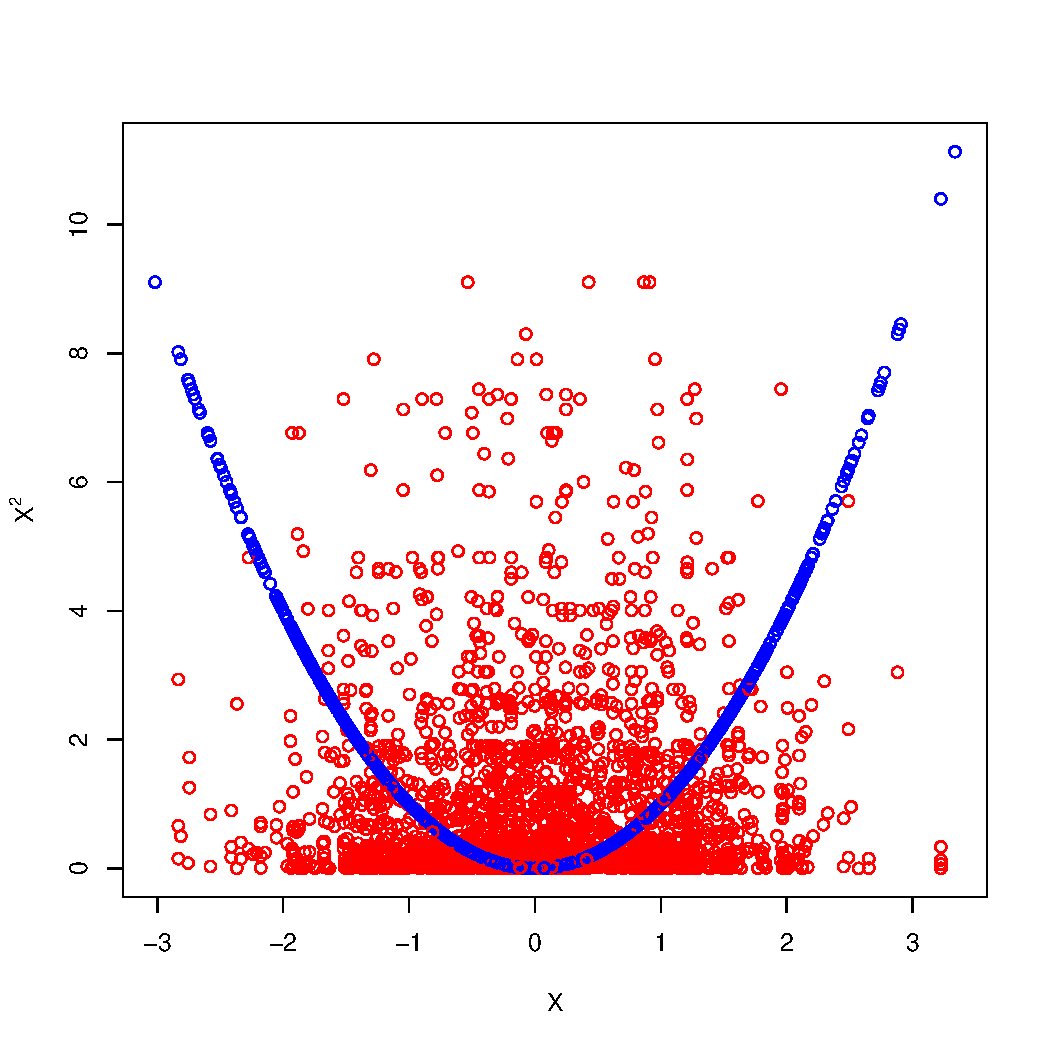
\includegraphics[scale=.55]{sepvar.pdf}
 \end{frame}
 
 %%%%
\begin{frame}
  \frametitle{Imputing squares: Option 2\&3}
   \begin{itemize}
   \item Impute, then transform
   \begin{itemize}
   \item Transform $X$ to $X^2$ in the imputed data. 
   \item Preserves the relation between $X$ and $X^2$ after imputation. 
   \item Yields heavily biased regression estimates (also under MCAR)
   \end{itemize}
   \item Passive imputation
   \begin{itemize}
   \item Computes $X^2$ each time $X$ is imputed. 
   \item Equivalent to `Impute, then transform'   
   \end{itemize}
  \end{itemize}
    \vspace{0.2 in}
\resizebox{\textwidth}{!}{  
\begin{tabular}{lcccccrl}
\hline
							&MCAR	&MARleft	&MARmid		&MARtail	& MARright\\
 \hline
%\textit{Polynomial combination}	&&&&&\\
%Intercept ($\alpha$)				&0		&-0.01	&-0.01	&-0.05	&-0.07\\
%Slope of $X$ ($\beta_1$)			&1		&1		&1		&0.96	&0.96\\	
%Slope of $X^2$ ($\beta_2$)		&1		&1		&1.01	&1.06	&1.09\\	
%Residual SD ($\sigma_\epsilon$) 	&1		&1		&1		&1.03	&1.05\\	
%$R^2$						&0.75	&0.75	&0.75	&0.73	&0.73\\\\
\textit{Impute, then transform}	&&&&&\\
Intercept ($\alpha$)				&0.39	&0.29	&0.26	&0.52	&0.56\\
Slope of $X$ ($\beta_1$)			&0.93	&0.94	&0.87	&1.01	&1.06\\
Slope of $X^2$ ($\beta_2$)		&0.61	&0.60	&0.67	&0.56	&0.66\\
Residual SD ($\sigma_\epsilon$) 	&1.48	&1.44	&1.41	&1.56	&1.62\\
$R^2$						&0.45	&0.48	&0.5		&0.39	&0.34\\
%\textit{Passive imputation}	&&&&&\\
%Intercept ($\alpha$)				&0.39	&0.29	&0.26	&0.52	&0.56\\
%Slope of $X$ ($\beta_1$)			&0.93	&0.94	&0.87	&1.01	&1.05\\
%Slope of $X^2$ ($\beta_2$)		&0.61	&0.60	&0.68	&0.56	&0.66\\
%Residual SD ($\sigma_\epsilon$) 	&1.48	&1.45	&1.41	&1.57	&1.62\\
%$R^2$						&0.45	&0.48	&0.50	&0.38	&0.34\\\\
%\textit{Transform, then impute}	&&&&&\\
%Intercept ($\alpha$)				&0		&0.19	&-0.13	&0.01	&-0.05\\
%Slope of $X$ ($\beta_1$)			&1		&0.91	&0.97	&1.14	&1.32\\
%Slope of $X^2$ ($\beta_2$)		&1		&0.91	&0.95	&1.14	&1.32\\
%Residual SD ($\sigma_\epsilon$) 	&1		&0.95	&1		&1.06	&1.15\\
%$R^2$						&0.75	&0.77	&0.75	&0.72	&0.67\\
\hline
\end{tabular}
}

 \end{frame}
 
  %%%%
\begin{frame}
  \frametitle{Proposal: bivariately impute $X$ and $X^2$}
    \begin{itemize}
  \item Polynomial combination imputation
  \begin{itemize}
  \item Do not impute $X$ and $X^2$ but rather impute the linear combination $Z=X\beta_1 + X^2\beta_2$
  \item Decompose the imputed linear combination $Z$ into the distinct real roots
  \begin{align*}
 X_-  &=-\frac{1}{2\beta_2} \left ( \sqrt{4\beta_2Z + \beta_1^2} +\beta_1 \right )
\\  X_+   &= \frac{1}{2\beta_2} \left ( \sqrt{4\beta_2Z + \beta_1^2}-\beta_1\right  )
\end{align*}
  \end{itemize}
  \end{itemize}
 \end{frame}
 
 %%%%
\begin{frame}
  \frametitle{Choosing a root}
  \vspace{-.05 in} %Control vertical offset
  \centering
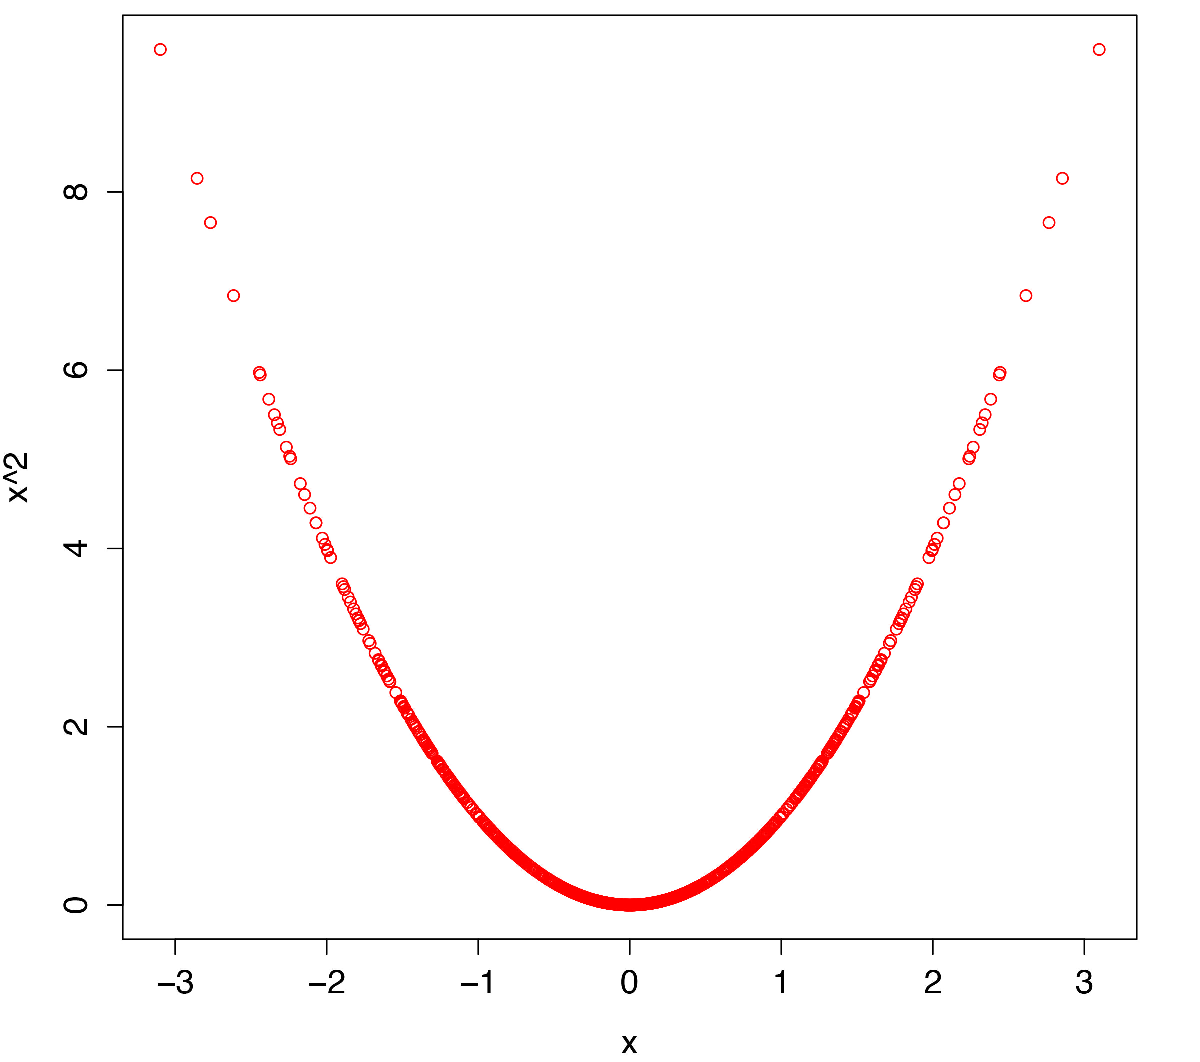
\includegraphics[scale=.45]{Chooseroots1.pdf}
 \end{frame}
 
  %%%%
\begin{frame}
  \frametitle{Choosing a root}
  \vspace{-.05 in} %Control vertical offset
  \centering
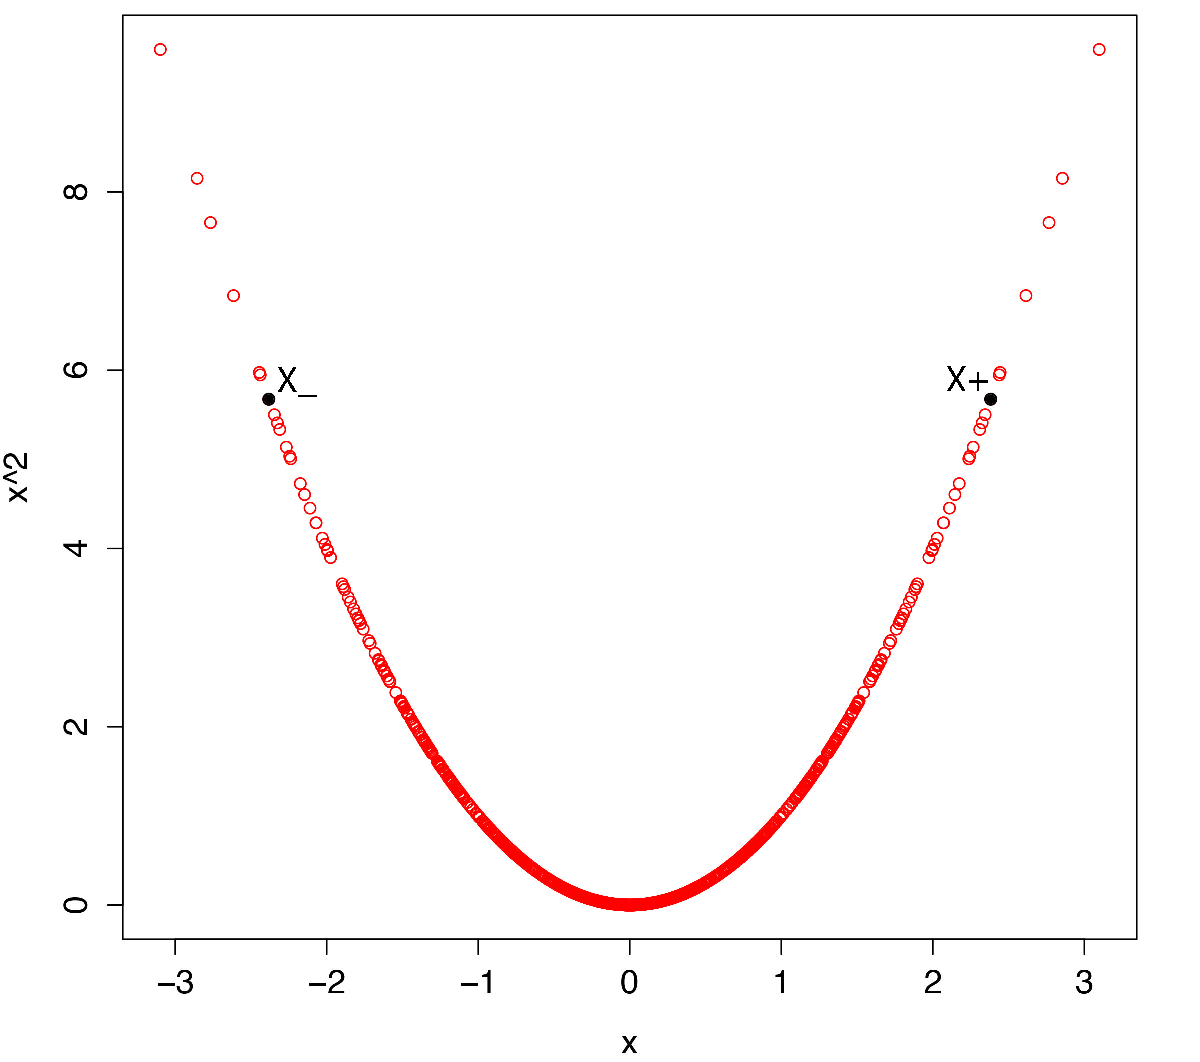
\includegraphics[scale=.45]{Chooseroots2.pdf}
 \end{frame}
 
   %%%%
\begin{frame}
  \frametitle{Choosing a root}
  \vspace{-.05 in} %Control vertical offset
  \centering
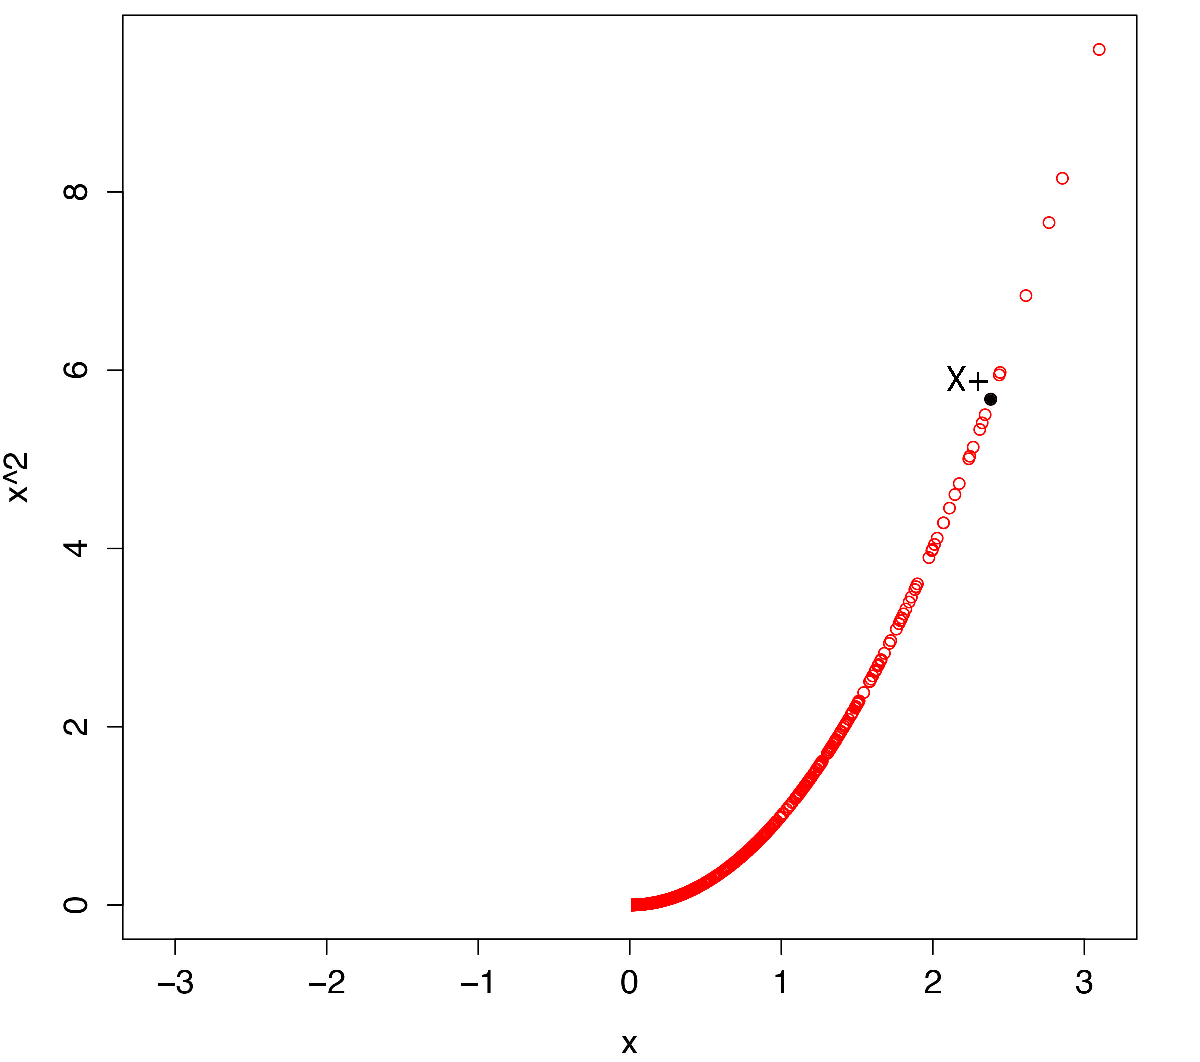
\includegraphics[scale=.45]{ChooseXplus.pdf}
 \end{frame}
 
 
   %%%%
\begin{frame}
  \frametitle{Choosing a root}
  \vspace{-.05 in} %Control vertical offset
  \centering
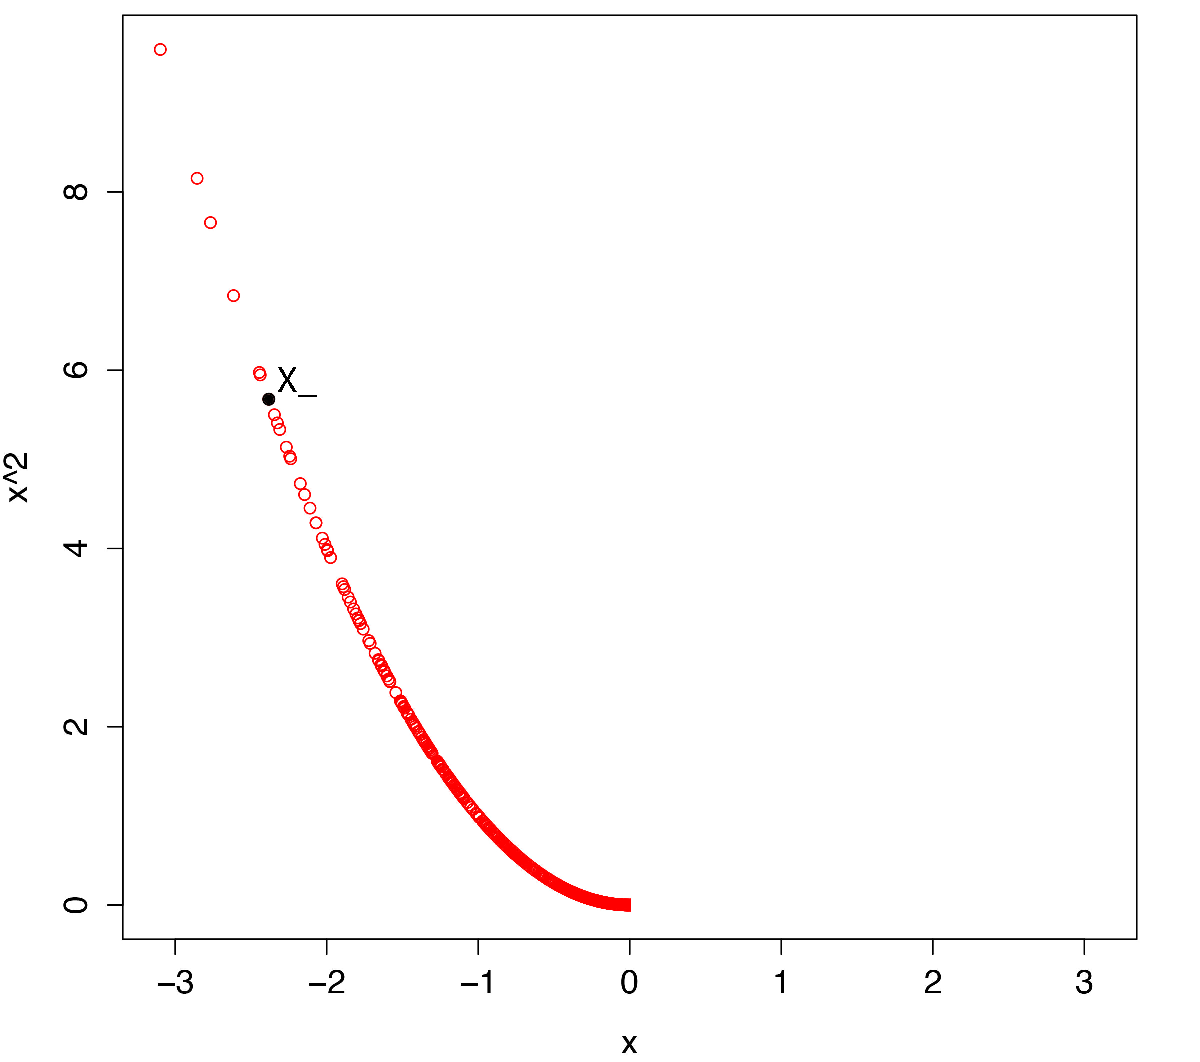
\includegraphics[scale=.45]{ChooseXmin.pdf}
 \end{frame}

   %%%%
\begin{frame}
  \frametitle{The minimum is located at $X_{min} =  -\beta_1/-2\beta_2$}
  \vspace{-.05 in} %Control vertical offset
  \centering
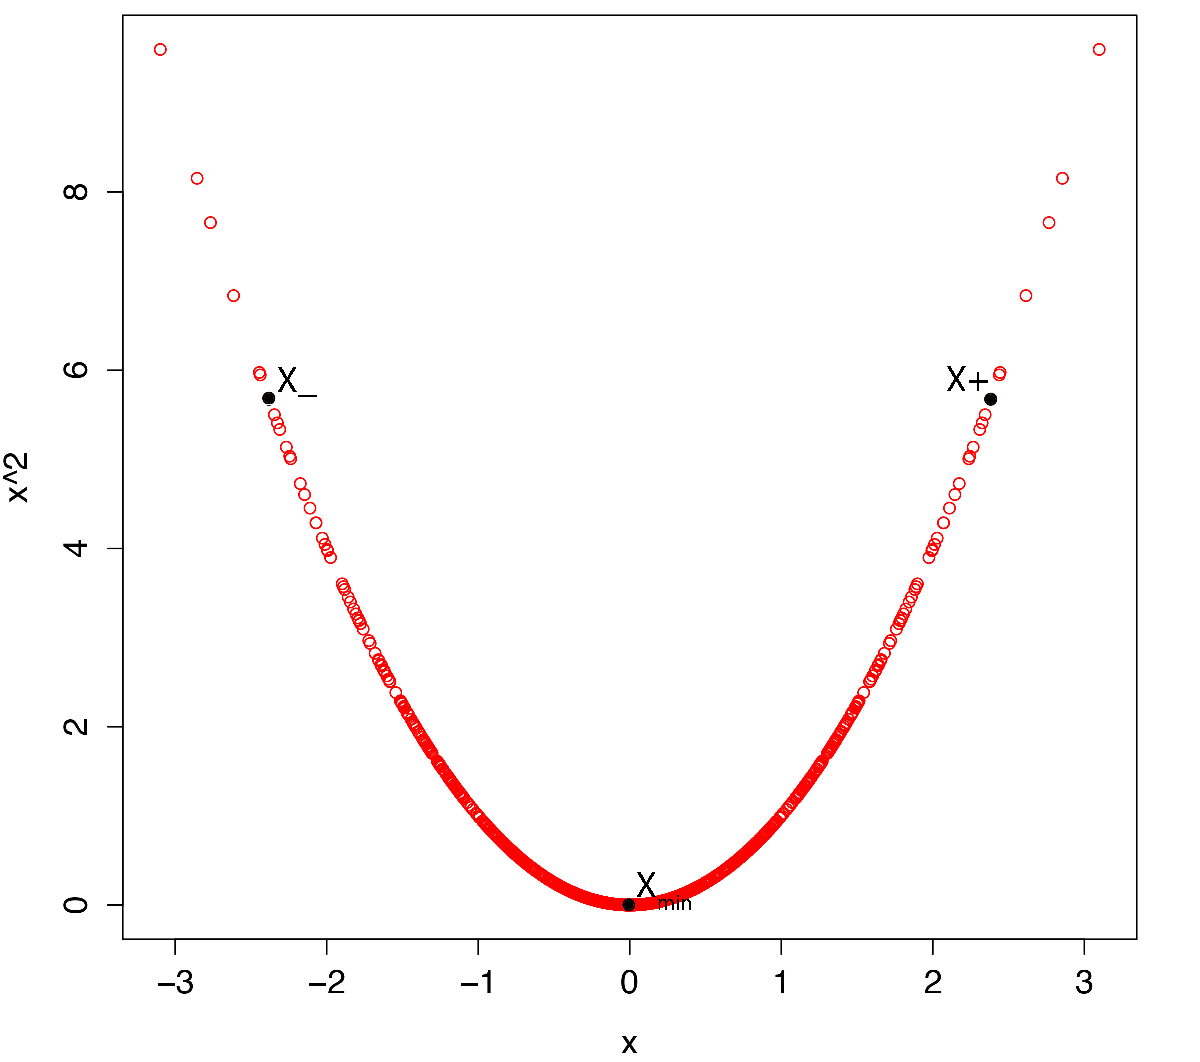
\includegraphics[scale=.45]{ChooseV.pdf}
 \end{frame}
 
    %%%%
\begin{frame}
  \frametitle{Create binary variable $V = (V_{obs}, V_{mis})$}
  \vspace{-.05 in} %Control vertical offset
  \centering
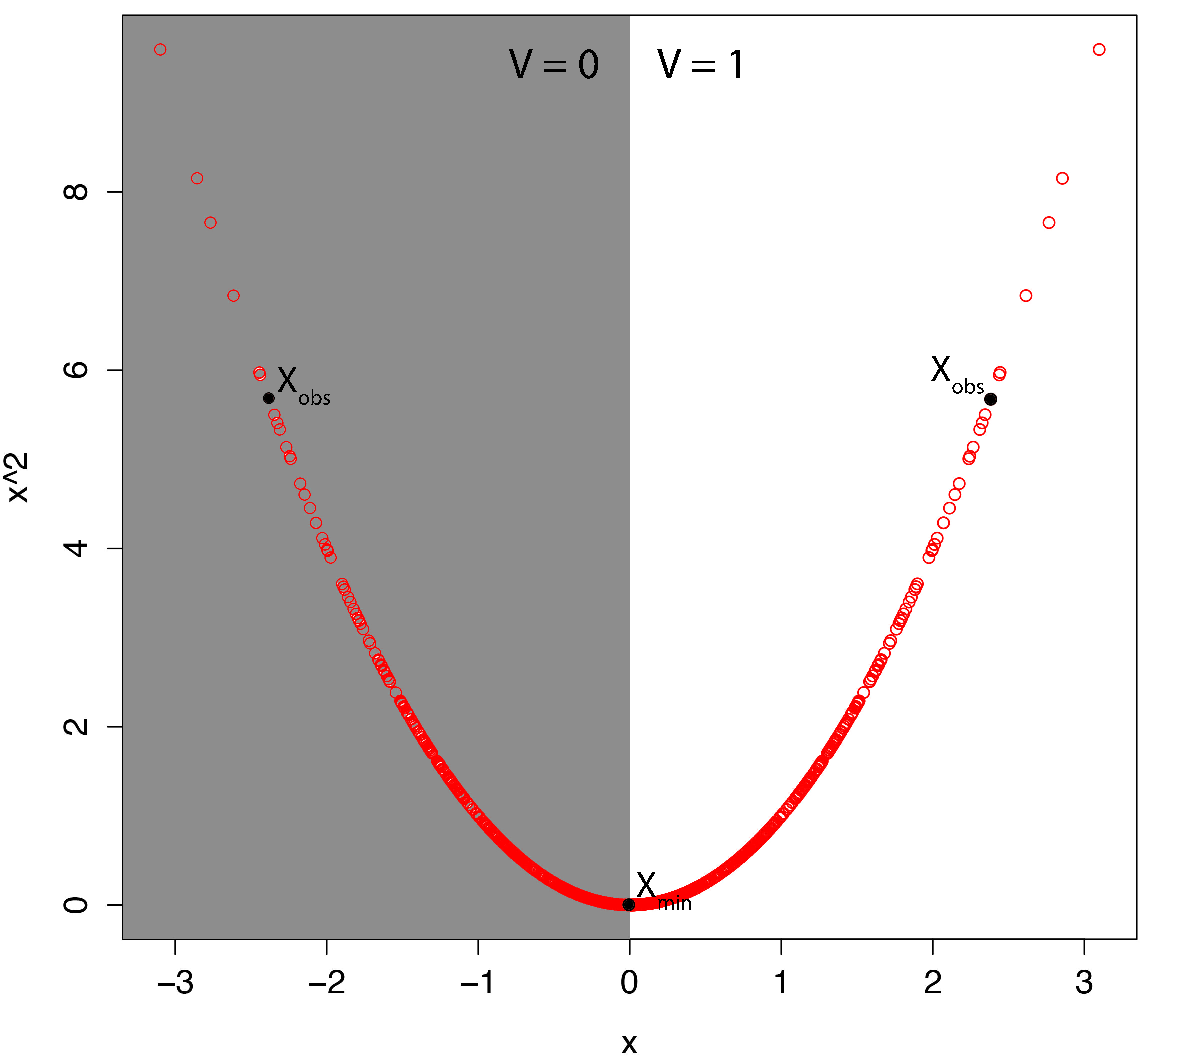
\includegraphics[scale=.45]{ChooseV2.pdf}
 \end{frame}
 
 %%%%
\begin{frame}
  \frametitle{Proposal: drawing roots with some probability}
    \begin{itemize}
    \item We can model the probability $V_{obs}$ for either arm on the observed $Z$ as
    \begin{equation*}\label{PV}
\textnormal{logit}P(V=1)=Y\beta_Y + Z\beta_Z + YZ\beta_{YZ}.
\end{equation*}
\item We can expand this model to obtain estimated (or imputed) probabilities $V_{mis}$ for imputed $Z$.
\item Sample either $X_-$ or $X_+$ by randomly drawing from the binomial distribution using the above probability. 
\item Calculate $X^2$ from the imputed $X$
  \end{itemize}
 \end{frame}
 
    %%%%
\begin{frame}
  \frametitle{Polynomial Combination}
  \vspace{-.45 in} %Control vertical offset
  \centering
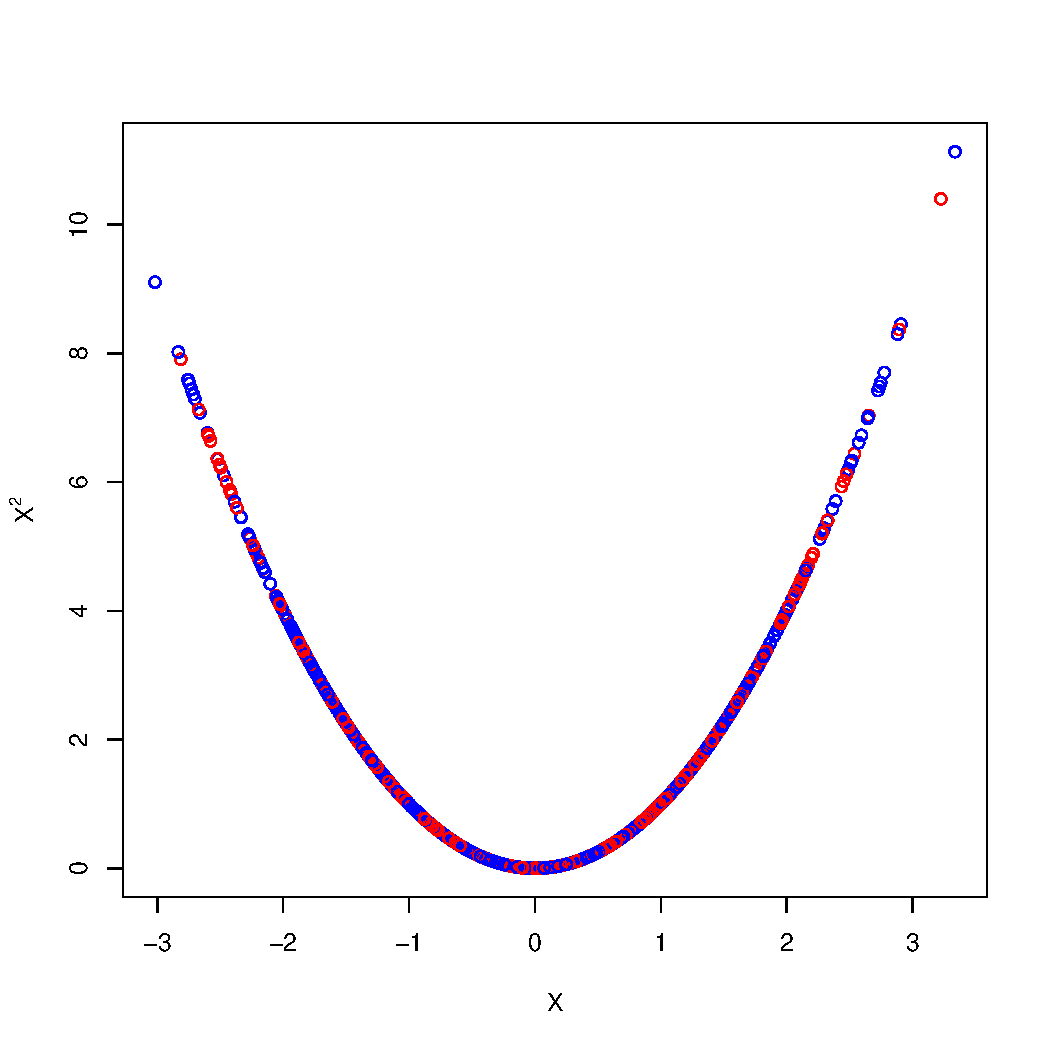
\includegraphics[scale=.55]{polycomb.pdf}
 \end{frame}
 
  %%%%
\begin{frame}
  \frametitle{Polynomial Combination}
    \begin{itemize}
  \item Yields unbiased regression estimates under MCAR and MAR
  \item Preserves the relation between $X$ and $X^2$ after imputation. 
  \item Easily applicable and already available in \texttt{mice}\footnote{ \tiny Stef van Buuren, Karin Groothuis-Oudshoorn (2011). mice: Multivariate Imputation by Chained Equations in R. Journal of Statistical Software, 45(3), 1-67.} in \texttt{R}\footnote{ \tiny R Core Team (2014). R: A language and environment for statistical computing. R Foundation for Statistical Computing, Vienna, Austria. URL http://www.R-project.org/.}
  \end{itemize}
      \vspace{0.2 in}
\resizebox{\textwidth}{!}{  
\begin{tabular}{lcccccrl}
\hline
							&MCAR	&MARleft	&MARmid		&MARtail	& MARright\\
 \hline
\textit{Polynomial combination}	&&&&&\\
Intercept ($\alpha$)				&0		&-0.01	&-0.01	&-0.05	&-0.07\\
Slope of $X$ ($\beta_1$)			&1		&1		&1		&0.96	&0.96\\	
Slope of $X^2$ ($\beta_2$)		&1		&1		&1.01	&1.06	&1.09\\	
Residual SD ($\sigma_\epsilon$) 	&1		&1		&1		&1.03	&1.05\\	
$R^2$						&0.75	&0.75	&0.75	&0.73	&0.73\\
\hline
\end{tabular}
}
\end{frame}
 
     %%%%
\begin{frame}
  Published as Vink, G., \& van Buuren, S. (2013). Multiple Imputation of Squared Terms. Sociological Methods \& Research, 42(4), 598-607.
 \end{frame}
\end{document}
